\documentclass[xcolor=dvipsnames]{beamer}
\usepackage[utf8x]{inputenc}
\usepackage{float}
\usepackage{graphicx}
\usepackage[absolute, overlay]{textpos}
\usepackage{multirow}

%%%%%%%%%%%%%%%%%%%%%%%%%%%%%%%%%%%%%%%%%%%%%%%%%%%
%				COLORS
%%%%%%%%%%%%%%%%%%%%%%%%%%%%%%%%%%%%%%%%%%%%%%%%%%%
\definecolor{darkgray}{RGB}{69, 69, 69}
\definecolor{darkblue}{RGB}{60, 34, 131}
\definecolor{lightpurple}{RGB}{154, 140, 191}

%%%%%%%%%%%%%%%%%%%%%%%%%%%%%%%%%%%%%%%%%%%%%%%%%%%
%				THEME SETTINGS
%%%%%%%%%%%%%%%%%%%%%%%%%%%%%%%%%%%%%%%%%%%%%%%%%%%
\usetheme{Dresden}
\setbeamercolor{normal text}{fg=darkgray}
\setbeamercolor{SupFooter}{bg=darkblue}

%%%%%%%%%%%%%%%%%%%%%%%%%%%%%%%%%%%%%%%%%%%%%%%%%%%
%				THEME TEMPLATES
%%%%%%%%%%%%%%%%%%%%%%%%%%%%%%%%%%%%%%%%%%%%%%%%%%%
\defbeamertemplate*{title page}{customized}[1][]{
    \centering
	\textbf{\usebeamerfont{title}\inserttitle}\par
	\usebeamerfont{subtitle}\insertsubtitle\par
	\vfill
	\usebeamercolor[fg]{subtitle}
	\small \usebeamerfont{author}\insertauthor\par
	\bigskip
	Superviseurss: Mme. Laurence Allencach
	\bigskip
	\usebeamerfont{institute}\insertinstitute\par
	\usebeamerfont{date}\insertdate\par
	\usebeamercolor[fg]{titlegraphic}\inserttitlegraphic
}

\newcommand{\unilogo}{
    \setlength{\TPHorizModule}{1pt}
    \setlength{\TPVertModule}{1pt}
    \begin{textblock}{1}(305,259)
        
\includegraphics[scale=0.088]{img/paris_13.jpg}
    \end{textblock}
}

\newcommand{\suplogo}{
    \setlength{\TPHorizModule}{1pt}
    \setlength{\TPVertModule}{1pt}
    \begin{textblock}{1}(8,8)
        
\includegraphics[scale=0.9]{img/sup_galilee.jpg}
    \end{textblock}
}

\defbeamertemplate{headline}{my header}{
    \vspace*{0.57cm}
	\suplogo
	\hspace*{2.5cm}
	\textbf{\large \insertsection}
	\vspace*{0.5cm}
}

\defbeamertemplate{footline}{my footer}{
    \begin{beamercolorbox}[ht=6ex]{SupFooter}
	    \vspace*{0.05cm}
	    \hspace*{0.3cm}
	    \textbf{\textcolor{lightpurple}{\large \insertframenumber /\inserttotalframenumber}}
        \hfill
	    \textbf{\textcolor{lightpurple}{\large www.sup-galilee.univ-paris13.fr}}
	    \hspace*{2cm}
	    \unilogo
    \end{beamercolorbox}
}
\setbeamertemplate{footline}[my footer]
\setbeamertemplate{headline}[my header]

%%%%%%%%%%%%%%%%%%%%%%%%%%%%%%%%%%%%%%%%%%%%%%%%%%%
%				TITLE DATA
%%%%%%%%%%%%%%%%%%%%%%%%%%%%%%%%%%%%%%%%%%%%%%%%%%%
\title[Enquête Industrielle]{Enquête Industrielle}
\subtitle{M. Alexandre Moyer : Ing\'enieur Conseil chez 
\includegraphics[scale=0.11]{img/logo_extia.jpg}}
\author[M. Kajioue, E. Ejangue, A. Fikl]{Mohamed Amine KAJIOUE \and Estelle EJANGUE \and Alexandru FIKL}

\begin{document}

\begin{frame}
	\maketitle
\end{frame}

\begin{frame}{Sommaire}
	\tableofcontents
\end{frame}

\section{L'entreprise : Extia}
\begin{frame}{Extia - Introduction}
\begin{itemize}[<+-| alert@+>]
    \item \textbf{Société de Conseil en Ingénierie} qui compte aujourd'hui plus de
300 consultants tous diplômés des Grandes Écoles d'Ingénieurs.
    \item Le groupe a été fond\'e en 2007 par Nicolas BOURDIN, Arnaud FREY et Patrick LETOVSKY
	\item Il est spécialisé dans 5 principaux secteurs :
	\begin{center}
	    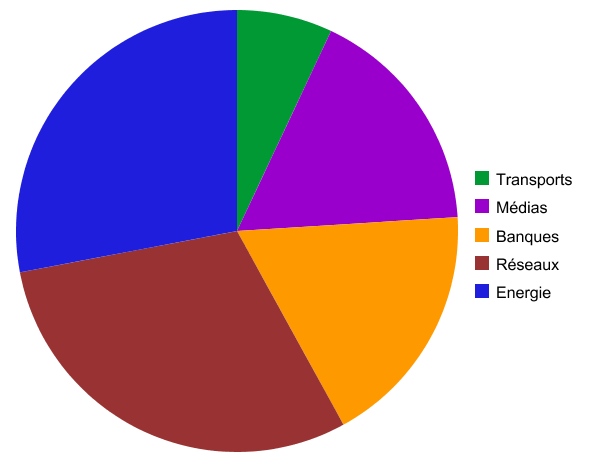
\includegraphics[scale=0.25]{img/extia_sectors.png}
	\end{center}
\end{itemize}
\end{frame}

\begin{frame}{Extia - Détails}
\begin{itemize}[<+-| alert@+>]
	\item La société a connu une croissance très rapide :
	\begin{center}
	    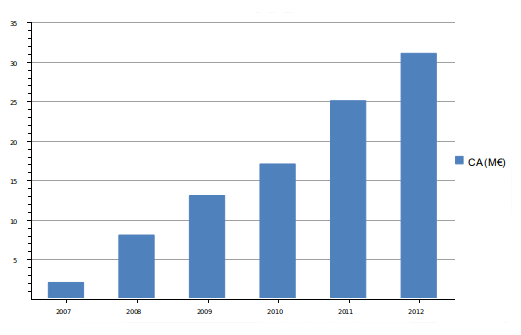
\includegraphics[scale=0.45]{img/extia-profit.png}
	\end{center}
    \item Elle a des filiales à \textbf{Ile-de-France} (EXTIA IDF, son siège social),
\textbf{Aix en Province} (EXTIA RHA) et \textbf{Lyon} (EXTIA PACA).
\end{itemize}
\end{frame}

\section{L'ingénieur : M. Alexandre Moyer}
\begin{frame}{Son parcours scolaire}
\begin{itemize}[<+-| alert@+>]
    \item \textbf{Alexandre Moyer} a obtenu son baccalauréat scientifique en 2000.
	\item Après trois années de classe préparatoire, il intègre Sup Galilée en
2003 ou il poursuit ses études dans la formation MACS.
    \item En septembre 2005 il a fait un semestre de quatre mois à \textbf{l'École
Polytechnique de Montréal}.
	\item Il a fait un stage de trois mois \`a \textbf{AMADEUS SAS} et après un autre
de six mois à \textbf{ONERA}.
\end{itemize}
\end{frame}

\begin{frame}{Son parcours en entreprises}
\begin{itemize}[<+-| alert@+>]
    \item L'entreprise \textbf{AMADEUS SAS} il intègre pour une durée de 3 mois.
    \item Par le biais d'une amie il intègre \textbf{l'INRIA} pour une durée de 18
mois.
	\item \`A INRIA Alexandre Moyer a contribué au développement de \textbf{DiscoGrid}, un logiciel qui permet
de partitionnement de maillages (grilles).
\end{itemize}
\end{frame}

\begin{frame}{A Extia I}
\begin{itemize}
    \item <+-| alert@+> Alexandre Moyer est intégré a EXTIA dans avril 2008 comme un Ingénieur
Conseil.
    \item <+-| alert@+> Dans les derniers quatre années il a conseillé pour beaucoup d'entreprises
telles que : France Telecom, Gaz de France et l'Institut Français du Pétrole.
\begin{columns}
  \begin{column}{0.5\textwidth}
    \centerline{
\includegraphics[scale=0.2]{img/francetelecom.jpeg}}
  \end{column}

  \begin{column}{0.3\textwidth}
    \centerline{
\includegraphics[scale=0.2]{img/gdf.jpeg}}
  \end{column}
\end{columns}
\begin{center}
    
\includegraphics[scale=0.2]{img/ifp.jpeg}
\end{center}

\end{itemize}
\end{frame}

\begin{frame}{A Extia II}
Les projets d'Alexandre Moyer à Extia :

\hbox{}

\footnotesize
\begin{tabular}{| l | p{6.5cm} |}
\hline
\textbf{France Telecom} & Modélisation pour le logiciel Odyssee (2008-2009)\\\hline
\multirow{2}{*}{\textbf{Gaz de France}} & $\bullet$ Recette d'un outil de diagnostic énergétique (2009)\\
 & $\bullet$ Développement d'un outil de diagnostic consommation (2009)\\\hline
\multirow{5}{*}{\textbf{Institut Français du Pétrole}} & $\bullet$ Développement des gradients analytiques pour les maillages CPG (2011)\\
& $\bullet$ Parallélisation du couplage fond surface (2011)\\
& $\bullet$ Redéfinition des tailles de blocs : une taille de bloc par maille (2010)\\
& $\bullet$ Développement d'un outil de tests de non-régression (2010)\\
& $\bullet$ Portage du simulateur de réservoir PumaFLOW sous Windows (2009)\\\hline
\end{tabular}
\end{frame}


\section{Conclusion}
\begin{frame}
\begin{itemize}
    \item Nous avons une meilleure idée quant à la spécialité que nous devrons choisir dans
les années à venir.
	\item Nous en savons plus sur le rythme de travail auquel nous serions éventuellement
confrontés.
	\item Nous avons découvert des domaines d'applications des Mathématiques Appliquées.
	\item Qualités propres a un ingénieur : la curiosité et l'ouverture d'esprit.
	\item De plus, cette démarche nous a appris à travailler en équipe.
\end{itemize}
\end{frame}

\begin{frame}
\begin{center}

\LARGE
\textbf{Merci beaucoup pour votre attention.}

\hbox{}

\Large
Passons aux questions !

\end{center}
\end{frame}

\end{document}
